\chapter{Erster Anhang - Technische Spezifikationen}
\label{Kap:Anhang1}
In diesem Anhang sind technische Spezifikationen und eine Grafik mit Entwicklung von Wirkungsgraden verschiedener PV-Technologien gelistet. Die Tabellen und abbildungen gliedern sich in die folgenden Sektionen.

\section{Entwicklung verschiedener PV-Technologien}

\begin{landscape}
  \begin{figure}[h]
      \centering
      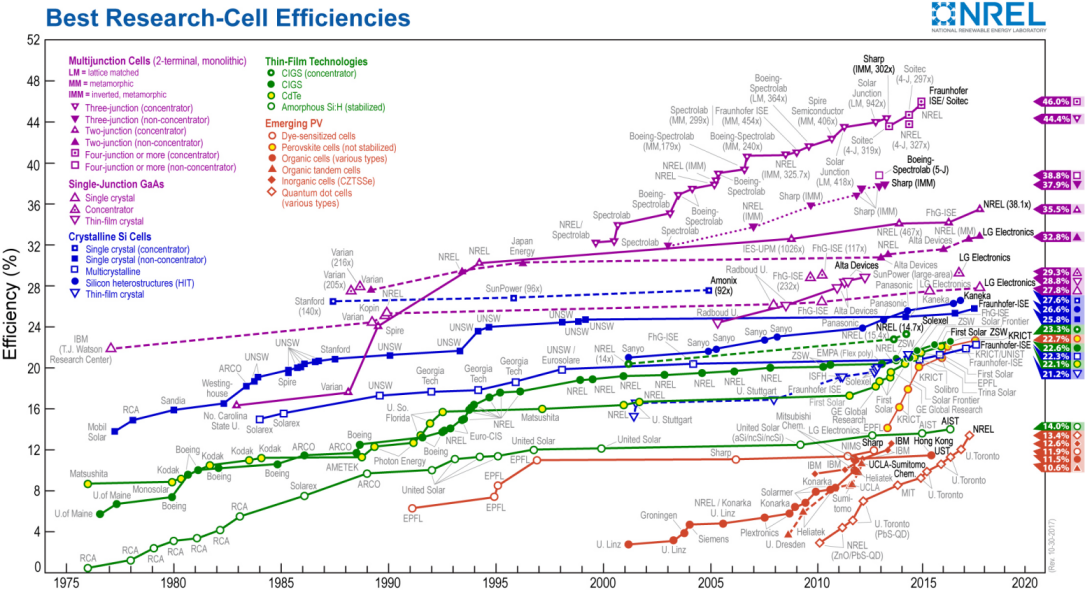
\includegraphics[width=\linewidth]{NREL_PV_efficiency_1975_2020}
      \caption{Entwicklung der Wirkungsgrade verschiedener Solarzellentechnologien \cite{Comparison_Batteries_2015}, \cite{NREL_PV_eta}}
      \label{Abb:Vgl_PV_eta}
  \end{figure}
\end{landscape}

\begin{landscape}
\section{Steckersysteme und Ladetechniken für Elektro-Autos}
  \begin{table}[h]
      \centering
      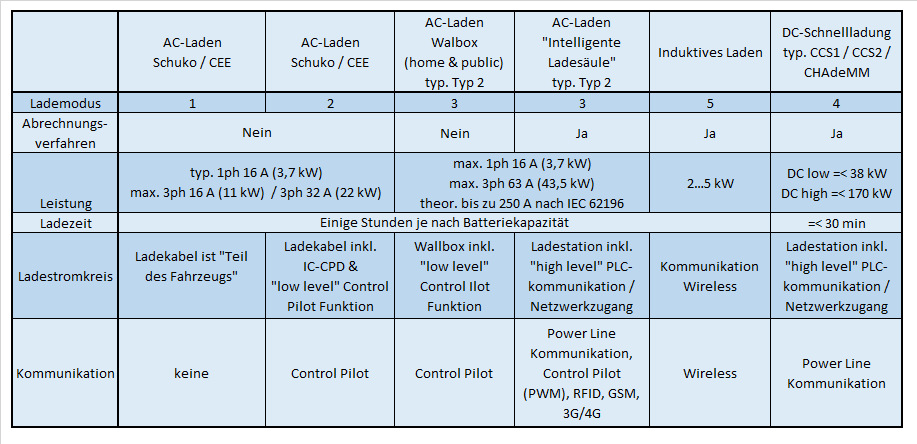
\includegraphics[width=0.9\linewidth]{Vergleich_Ladesysteme_EAuto}
      \caption{Vergleich verschiedener Ladesysteme für E-Autos \cite[S.15]{Emobility_StatusQuo_2016}} 
      \label{Tab:Vgl_Ladesysteme_EAuto}
  \end{table}
\end{landscape}

  \begin{table}[h]
      \centering
      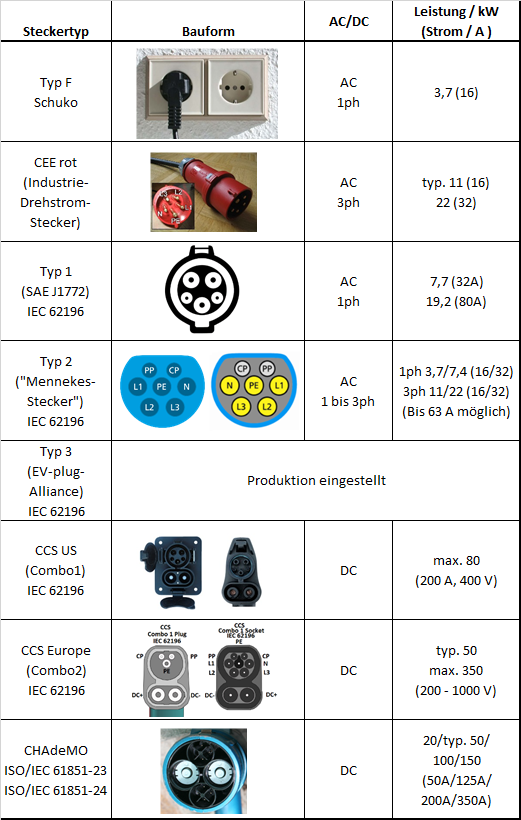
\includegraphics[width=14cm]{Stecker_typentabelle}
      \caption{Vergleich verschiedener standardisierter Steckervorrichtungen; Bildquellen:\cite{Abb_Steck_Schuko}\cite{Abb_Steck_CEE}\cite{Abb_Steck_Typ1}\cite{Abb_Steck_Typ2}\cite{Abb_Steck_Combo1}\cite{Abb_Steck_Combo2}\cite{Abb_Steck_CHAdeMO}}
      \label{Tab:Vgl_Steckervorrichtungen}
  \end{table}	

\begin{landscape}
\section{EEBUS Spezifikation}
  \begin{figure}[h]
      \centering
      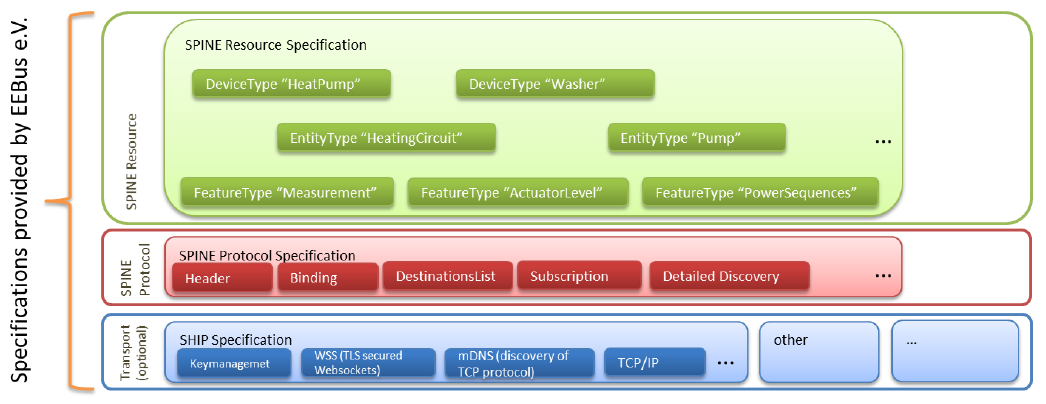
\includegraphics[width=\linewidth]{EEBUS_Spec}
      \caption{EEBUS Spezifikation im Detail \cite[S.5]{EEBUS_Intro}}
      \label{Abb:EEBUS_Spec}
  \end{figure}			
\end{landscape}                

\section{Herstellerangaben zu PV-Anlage, PV-Wechselrichter und Pufferbatterie}
\label{Kap:datasheet_pv_wr}

  \begin{figure}[h] 
      \centering
      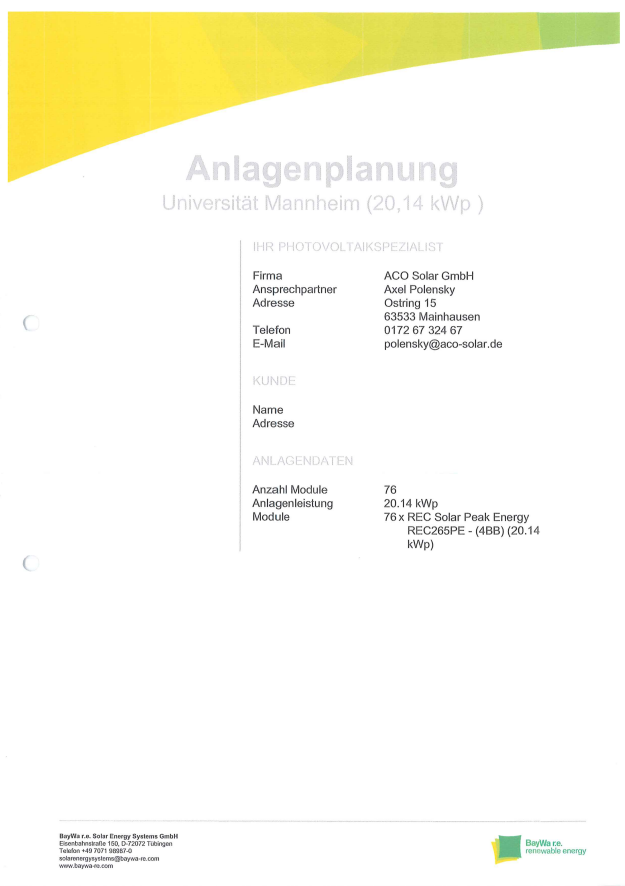
\includegraphics[width=0.8\linewidth]{datasheet_pv_1}
      \caption{Spezifikation der PV-Anlage auf Gebäude C der Hochschule Mannheim, Ausschnitt der Anlagenplanung} 
      \label{Abb:datasheet_pv_1}
  \end{figure} 	

  \begin{figure}[h] 
      \centering
      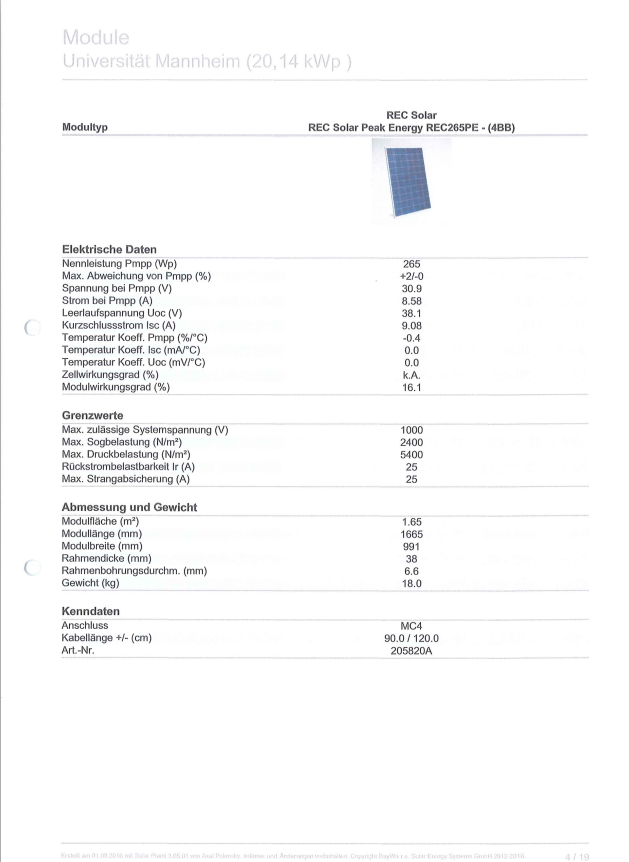
\includegraphics[width=\linewidth]{datasheet_pv_2}
      \caption{Spezifikation der PV-Anlage auf Gebäude C der Hochschule Mannheim, Ausschnitt der Anlagenplanung: Kenndaten des Moduls REC Solar Peak Energy REC265PE} 
      \label{Abb:datasheet_pv_2}
  \end{figure} 	

  \begin{figure}[h] 
      \centering
      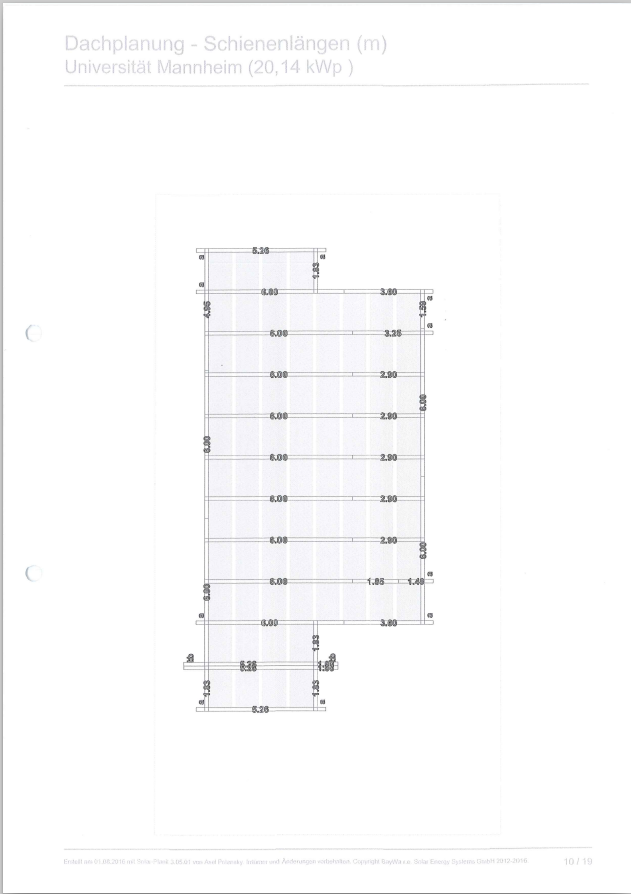
\includegraphics[width=\linewidth]{datasheet_pv_3}
      \caption{Spezifikation der PV-Anlage auf Gebäude C der Hochschule Mannheim, \\ Ausschnitt der Anlagenplanung: Dachplanung - Schienenlänge, Modulpositionen \\ (Himmelsrichtung Norden, oben im Bild)} 
      \label{Abb:datasheet_pv_3}
  \end{figure} 	

  \begin{figure}[h] 
      \centering
      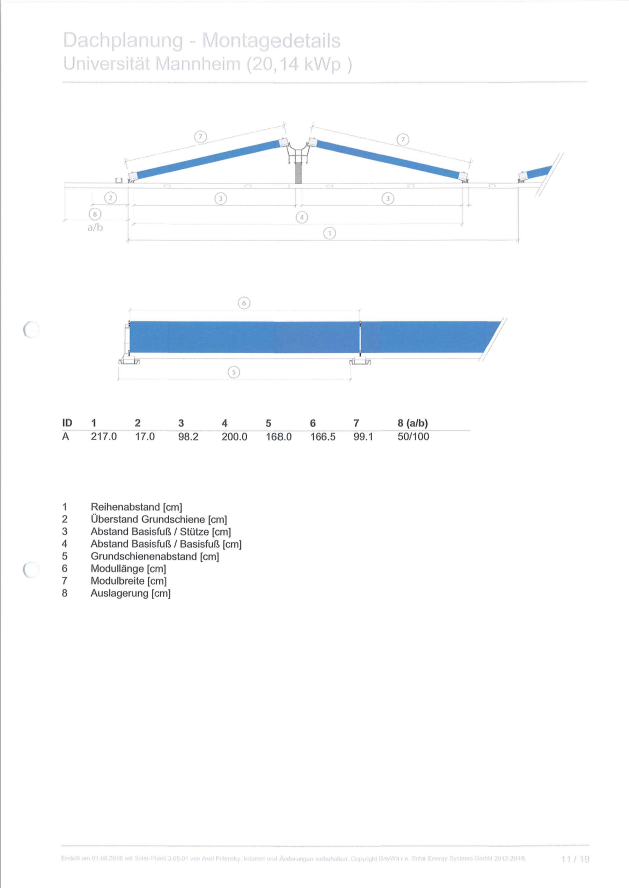
\includegraphics[width=\linewidth]{datasheet_pv_4}
      \caption{Spezifikation der PV-Anlage auf Gebäude C der Hochschule Mannheim, \\ Ausschnitt der Anlagenplanung: Dachplanung - Montagedetails, Modulneigung \\ (Westen links, Osten rechts im Bild)} 
      \label{Abb:datasheet_pv_4}
  \end{figure} 	

  \begin{figure}[h] 
      \centering
      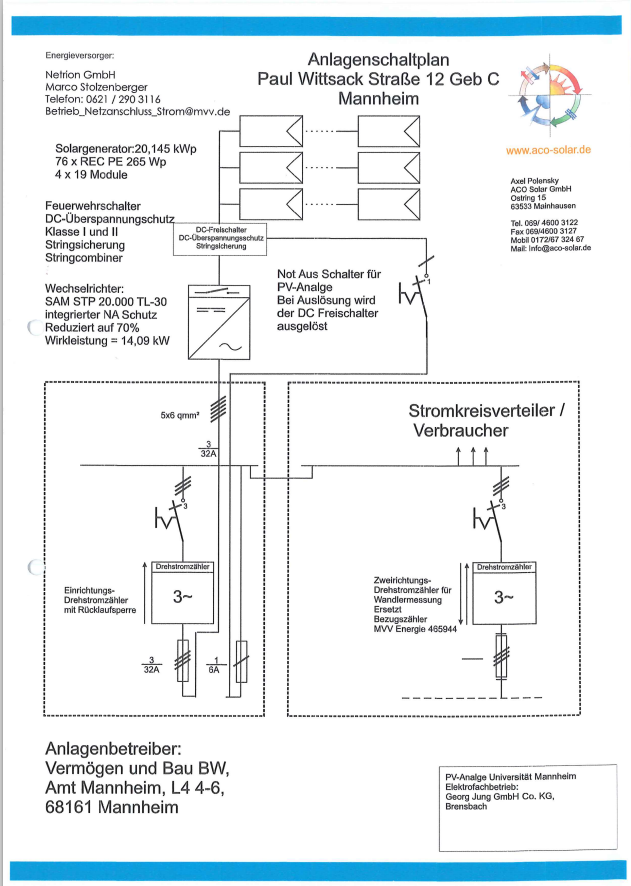
\includegraphics[width=\linewidth]{datasheet_pv_5}
      \caption{Spezifikation der PV-Anlage auf Gebäude C der Hochschule Mannheim, \\ Ausschnitt der Anlagenplanung: Anlagenschaltplan} 
      \label{Abb:datasheet_pv_5}
  \end{figure} 	

  \begin{figure}[h] 
      \centering
      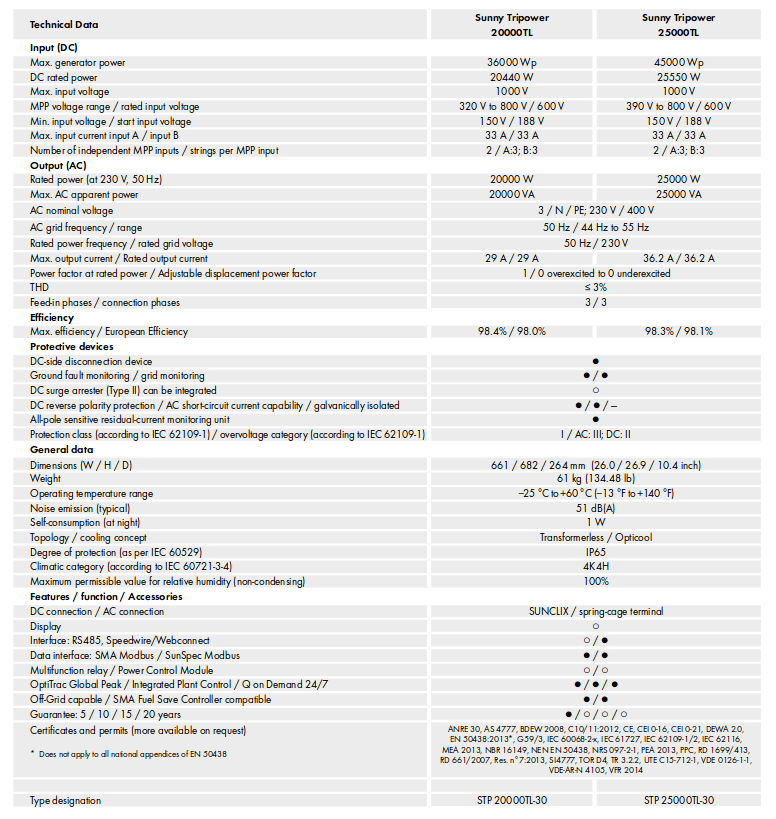
\includegraphics[width=\linewidth]{datasheet_wr}
      \caption{Spezifikation des PV-Wechselrichters, technische Herstellerangaben \cite{spec_SMA}} 
      \label{Abb:datasheet_wr}
  \end{figure} 	

  \begin{figure}[h] 
      \centering
      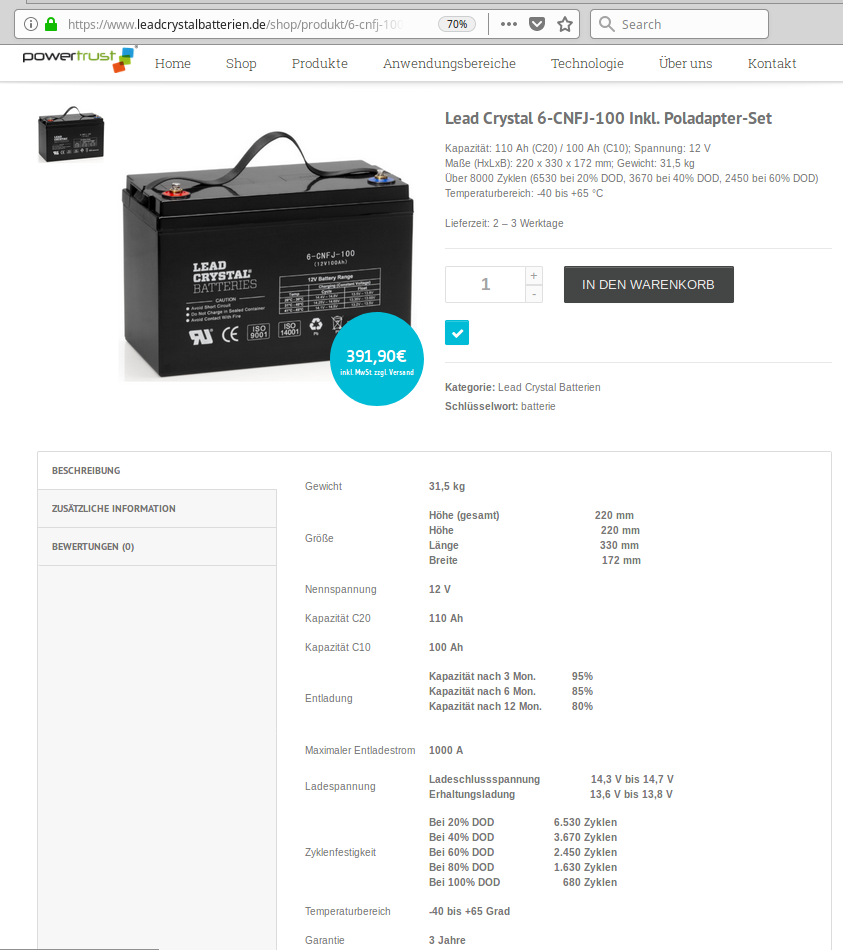
\includegraphics[width=\linewidth]{datasheet_akku}
      \caption{Spezifikation des Bleikristallakkus Lead Crystal 6-CNFJ-100 inkl. Poladapter-Set des Herstellers $\text{Lead Crystal}^{\textsuperscript{\textregistered}} ~\text{Batteries}$ \cite{spec_battery_buffer}}   
      \label{Abb:datasheet_akku}
  \end{figure} 	

  \begin{figure}[h] 
      \centering
      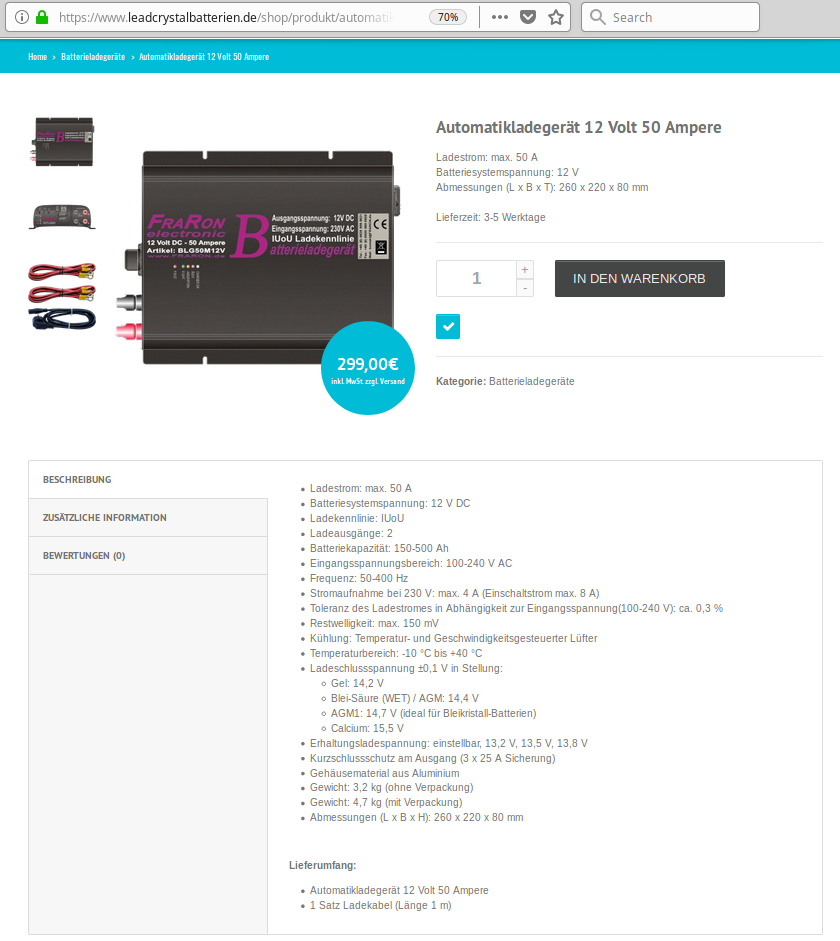
\includegraphics[width=\linewidth]{datasheet_laderegler}
      \caption{Spezifikation des Automatikladegeräts 12 Volt 50 Ampere des Herstellers Fraron \cite{spec_laderegler}} 
      \label{Abb:datasheet_laderegler}
  \end{figure} 	

\section{Projektplanung Gantt Chart}
\begin{landscape}
  \begin{figure}[h] 
      \centering
      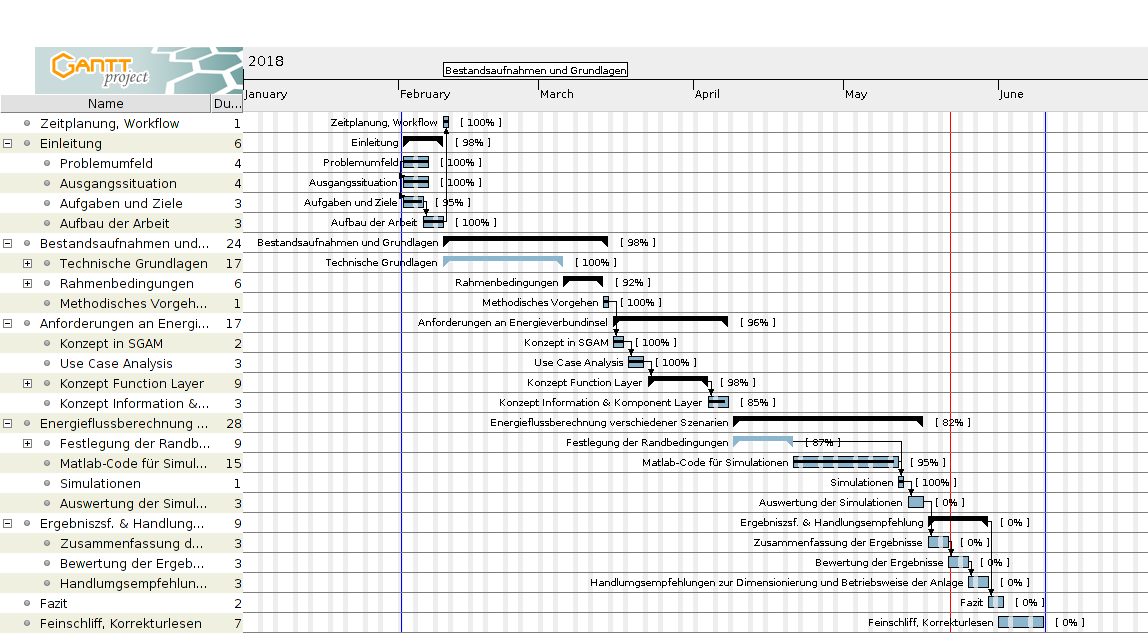
\includegraphics[width=0.8\linewidth]{Projektplanung}
      \caption{Projektplanung mit Gantt project}
      \label{Abb:gantt}
  \end{figure} 	
\end{landscape}